\documentclass[conference]{IEEEtran}
\IEEEoverridecommandlockouts
% The preceding line is only needed to identify funding in the first footnote. If that is unneeded, please comment it out.
\usepackage{cite}
\usepackage{amsmath,amssymb,amsfonts}
\usepackage{algorithmic}
\usepackage{graphicx}
\usepackage{textcomp}
\usepackage{xcolor}
\def\BibTeX{{\rm B\kern-.05em{\sc i\kern-.025em b}\kern-.08em
    T\kern-.1667em\lower.7ex\hbox{E}\kern-.125emX}}
\begin{document}

\title{Predicting the Average Two-Year Win Probability and Hire Tenure of NFL Head Coach Hires: Three Approaches}

\author{\IEEEauthorblockN{Jon C. Williamson}
\IEEEauthorblockA{\textit{Dept. of Computer Science \& Engineering} \\
\textit{Texas A\&M University}\\
College Station, TX, USA \\
jonwilliamson@tamu.edu}
}

\maketitle

\begin{abstract}
This project implemented regularized linear models, XGBoost models, and Multi-layer perceptron models to predict the average two-year winning probability and coach tenure classifications of head coach hires throughout the history of the NFL. The three probability regressions were not able to predict winning probability appreciably better than a model that only guesses the expected probability. These findings suggest that the features in this project, primarily driven by characteristics of the head coach, are not sufficient to predict a team's winning probability. In other words, it appears that a head coach hire will not drive a change in win probability based on these features. Two tenure classification models showed predictive ability with OVR AUROC values of 0.706 and 0.704. This performance shows that the features in this project do have some ability to predict the tenure of head coach hires.

\end{abstract}

\begin{IEEEkeywords}
machine learning, neural networks, prediction methods, supervised learning, unsupervised learning
\end{IEEEkeywords}

\section{Introduction}
Although the National Football League (NFL) is not publicly traded, evaluation of its teams suggests that it is worth over \$91 billion dollars \cite{b1}.  Equivalently, the average NFL franchise is worth \$2.86 billion dollars \cite{b1}. Despite these large evaluations, hiring successful head coaches is anything but repeatable in the NFL. In 2016, the median head coach tenure in position was three years \cite{b2}. Although this length is marginally better than other sports leagues \cite{b2}, comparing the average top job tenure to public sector best practice shows immense area for improvement. A publicly-traded company that changed CEOs at this rate would have an extremely volatile stock price and likely decreased stock demand \cite{b3}. In this analogy, the general manager is the entire Board of Directors. Moreover, successful head coach hiring is tremendously valuable, as a differentiated NFL head coach can bring about lasting success and divisional dominance, subsequently increasing the historical importance of a franchise and improving its bottom line. A machine learning model that can increase the hit probability of head coaching hires has the potential to add immense value to NFL franchises. This project attempts to predict two outcomes of head coach hires: the average two-year winning percent and the hire tenure, using three machine learning approaches.

\section{Literature Review}
There have been no journal publications that attempt to predict the success of NFL coaching hires through statistical learning techniques. Currently, the NFL is only beginning to implement artificial intelligence (AI) in play calling prediction \cite{b4}. Additionally, there are few papers that examine the impact of individual features on NFL head coaching success. Reference \cite{b5} used a linear regression with seven features to attempt to predict the number of wins of head coaches in their first three years in order to understand if prior NFL head coaching experience impacts success in position. This paper found that a previous head coaching experience had a negative impact on the success of new head coaches. Despite this finding, the model supported an adjusted $R^2$ of only $0.336$. This low value, the lack of regularization, and the small number of features  decreases confidence in the study's findings. Reference \cite{b6} reviews research in sports economics and suggests that hiring decisions made solely on playing success are unlikely to be optimal given financial (resource) inequality among sports franchises. 

\section{Problem Formulation}
This project develops three implementations of two machine learning models. The first model attempts to predict a coach's average winning probability in their first two years following hiring using three separate regressors. The second model attempts to predict the classification of coach tenure following hiring using three multi-class classifiers. Although the feature set and data points for these problems are largely identical, this report will analyze both models separately.

\section{Proposed Solution}

\subsection{Predicting Average Two-Year Winning Probability}
Equation \eqref{eq1} defines the calculation of average winning probability, $p_{win}$, as a function of the number of wins, $n_{wins}$, the number of losses, $n_{losses}$, and the number of ties, $n_{ties}$, of a head coach over any interval. 

\begin{equation}
        p_{win}=\frac{n_{wins} + 0.5*n_{ties}}{n_{wins} + n_{losses} + n_{ties}}
        \label{eq1}
\end{equation}

This winning probability is bound within $[0, 1]$. Predicting this continuous value requires regression. This project implements three regressors to attempt this prediction: 
\begin{enumerate}
  \item Linear Regression with Lasso Regularization\cite{b7}
  \item XGBoost Regressor\cite{b8}
  \item Multi-layer Perceptron (MLP) Regressor\cite{b7}
\end{enumerate}

The first implementation of this model is a simple linear model with $\ell_1$ norm regularization. This project uses $\ell_1$ regularization due to its tendency to remove features from the model. The second implementation of the model is an XGBoost regressor. This regressor uses gradient boosting to build a single predication model through the aggregation of weak learners. This project uses trees as the universal model for the XGBoost weak learners. The third and final implementation of this model is through a multi-layer perceptron regressor. This regressor is a basic neural network with a final regression node. It extracts features without supervision. This project utilizes extensive cross-validation to determine the optimal values for hyperparameters for each model implementation. 

This project uses root mean squared error (RMSE) as the evaluation metric for these regression models. This metric was chosen for two reasons. Firstly, its dimensions are identical to the dimensions of the prediction variable. Secondly, it punishes outliers greater than absolute error. It is important to note that the thresholds that constitute `good' and `bad' RMSE are impacted by the scale of the prediction. As a result, this project compares model RMSE against the RMSE for predicting the expected outcome to understand model performance. 


\subsection{Predicting Coach Tenure Classification}
This project defines the tenure of a coach hire as the number of years the hired coach remains in the same position before being fired, leaving, or retiring. A model that predicts this tenure directly would require regression. This level of granularity is not necessary, as there is no meaningful difference between a coach that is in position for ten years and one that is in position for twelve years. As a result, this project maps coach tenures to four tenure classifications in order to convert this problem to a classification. Equation \eqref{eq2} shows the mapping between the coach tenure, $t$, and coach tenure classification label, $C(t)$.
\begin{equation}
        C(t)=
        \begin{cases}
            0 &t \leq 2 		\\
            1 &2 < t \leq 4 \\
            2 &4 < t \leq 7 \\
            3 &t > 7
        \end{cases}
        \label{eq2}
\end{equation}

Equation \eqref{eq2} shows four independent coach tenure classification labels. The shortest tenure class, of one and two years, is intended to capture the worst head coach hires. The next class, of three and four years, is intended to capture coaches that are mediocre, i.e., coaches that teams would be happy to move on from but are not obligated to do so. The third coach tenure class is intended to capture successful head coaches with tenure between five and seven years. The fourth and final class is intended to capture the best coach hires in the history of the NFL, e.g., the Bill Belichick's and Don Shula's of the league.

This model seeks to predict the coaching tenure classification of head coach hires based on statistics available at the time of hiring. This project utilizes three implementations of this model:
\begin{enumerate}
  \item Logistic Regression with Lasso Regularization\cite{b7}
  \item XGBoost Classifier\cite{b8}
  \item Multi-layer Perceptron Classifier\cite{b7}
\end{enumerate}
These implementations are analogous to the three models in the previous subsection. The primary difference is that these implementations are classification models and not regression models. As with the previous model, this project utilizes extensive cross-validation to determine hyperparameter values for each implementation. This project uses macro-averaged one-versus-rest (OVR) area under the receiver operating characteristic curve (AUROC) to measure model performance. This performance metric  accounts for class imbalance.

\section{Data Description}
This project utilizes 25 features, two description labels, and the two model outputs for each head coaching hire. The two descriptive labels are the coach name and the hire year. These labels exist only to better understand the results and are not included in the prediction method of any model. Table \ref{tab1} shows the 25 features used in each model. Abbreviations included in feature descriptions include offensive coordinator (OC), defensive coordinator (DC), and head coach (HC).

\begin{table}[htbp]
\caption{Model Feature List}
\begin{center}
\begin{tabular}{|c||l|}
\hline
\textbf{No.} & \textbf{Description} \\
\hline
\hline
1 & Age at hiring \\
\hline
2 & Number of times previously hired as head coach \\
\hline
3 & Number of years’ experience as college position coach \\
\hline
4 & Number of years’ experience as college coordinator \\
\hline
5 & Number of years’ experience as college head coach \\
\hline
6 & Number of years’ experience as NFL position coach \\
\hline
7 & Number of years’ experience as NFL coordinator \\
\hline
8 & Number of years’ experience as NFL head coach \\
\hline
9 & Demotion presence in hiring history \\
\hline
10 & During years as NFL OC, team’s avg. norm. yardage rank \\
\hline
11 & During years as NFL OC, team’s avg. norm. point rank \\
\hline
12 & During years as NFL OC, team’s avg. norm. giveaway rank \\
\hline
13 & During years as NFL DC, team’s avg. norm. yardage rank \\
\hline
14 & During years as NFL DC, team’s avg. norm. point rank \\
\hline
15 & During years as NFL DC, team’s avg. norm. turnover rank \\
\hline
16 & During years as NFL HC, team’s avg. norm. yardage differential\\
&rank \\
\hline
17 & During years as NFL HC, team’s avg. norm. point differential \\
&rank \\
\hline
18 & During years as NFL HC, team’s avg. norm. turnover ratio rank \\
\hline
19 & Hiring team’s avg. winning percent in previous two years \\
\hline
20 & Hiring team’s avg. norm. turnover ratio rank in previous two \\
&years \\
\hline
21 & Hiring team’s avg. norm. point differential rank in previous\\
& two years \\
\hline
22 & Hiring team’s avg. norm. yard differential rank in previous\\
&two years \\
\hline
23 & Hiring team’s avg. norm. divisional placement in previous two\\
&years \\
\hline
24 & Hiring team’s number of playoff appearances in previous\\
&two years \\
\hline
25 & Hiring team’s number of playoff wins in previous two years \\
\hline
\end{tabular}
\label{tab1}
\end{center}
\end{table}

Table \ref{tab1} shows that features 1 through 18 are characteristics of head coaches at time of hiring, while features 19 through 25 are characteristics of the hiring team. This distinction is essential, as resource inequality among franchises does impact team success independent of any coaching effort \cite{b6}. Moreover, this project includes these team-specific features because the models could determine profiles of successful coaches with respect to team state in order to maximize win total and coach tenure. All features are purely numeric. Only one feature, feature 9, is categorical. All other features are continuous.

Features 10 through 18 and 20 through 23 reference average normalized team ranks in different categories. For these features, the single feature value is taken as the average of the normalized ranks for all years that qualify. A single normalized rank prior to averaging for these features is of the form $x \text{ out of }z$, where $x$ is the rank of the attribute by team out of $z$ total teams. Equation \eqref{eq3} linearly distributes the feature instance value, $f(x,z)$, from $1$ at the best rank to $0$ at the worst rank:

\begin{equation}
        f(x,z) = \frac{z-x}{z-1}
        \label{eq3}
\end{equation}

This rank normalization also allows coaches across eras to be compared, as performance is purely comparative to other teams in the same era. Raw data was collected by scraping pro-football-reference.com. The crawling script extracted three performance tables for all head coaches in NFL history. For any coach, these three tables detail the top-level coaching results, the team's ranks in many categories relative to the league, and the coach's career hiring record for every year in their career. 

The crawling script also extracted two performance tables for all franchises in NFL history. For any franchise, these two tables include the team's record \& ranks and playoff statistics for every season in franchise history.

A script was written to analyze the crawled data to extract the feature set and calculate the two model outputs for all coach hires in NFL history. It should be noted that this script considers interim promotions acts of coach hiring, as exceptional performance as an interim coach can lead to a non-interim promotion. This script identified 693 hiring instances in the history of the NFL.

Fig. \ref{fig1} shows the correlation matrix among all 25 features. This matrix shows that the data is not highly correlated. The three-by-three white boxes in the matrix show that there is no correlation among features 10 through 12 and 13 through 15. Features 10 through 12 are based on team performance as an offensive coordinator, while features 13 through 15 are from performance as a defensive coordinator. No coaches in the set were both an OC and a DC prior to being hired, hence there is no correlation value among those features. It should be noted that the feature set is somewhat sparse. All data is mean-imputed prior to being fed into any model.

\begin{figure}[htbp]
\centerline{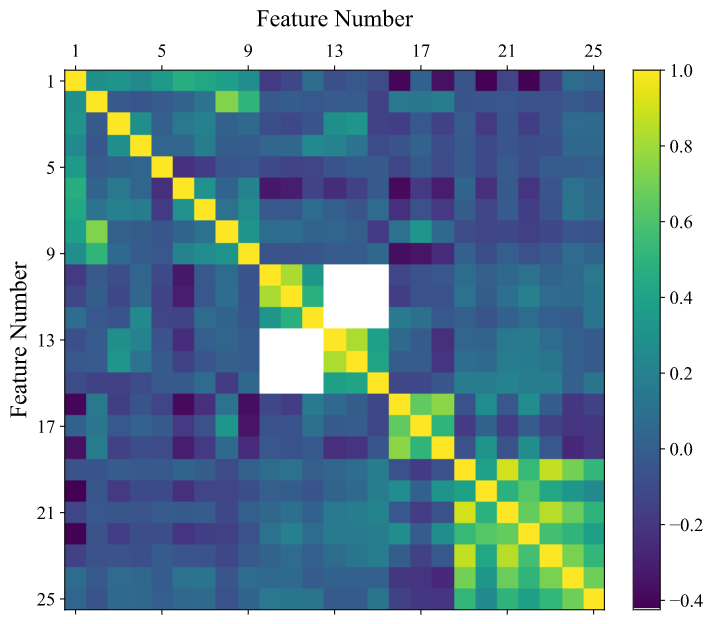
\includegraphics[width=1\linewidth]{corr.png}}
\caption{Feature correlation matrix.}
\label{fig1}
\end{figure}

There is some correlation among features 19 through 25. Recall that these features are characteristics of hiring teams in the two years prior to the coaching hire. It makes some sense that these features are correlated, as teams that perform well in these ranking metrics are likely better teams, and thus, should perform well in other ranking metrics. Lastly, there is correlation between feature 1, age at hiring, with features 2-9, which measure number of years of coaching experience at varying levels. This observed correlation is expected. 

Fig. \ref{fig2} shows a histogram of the two-year average winning probability for the data set. This figure shows that the mean average two-year winning percent for new head coach hires is $0.408$. The data is somewhat normally distributed. It should be noted that the outlying win probabilities are most often a result of interim head coach hires that were not promoted following the completion of the season. These coaches have a smaller sample size for win probability calculation, and thus can achieve extreme win probabilities that are more rare over the course of two complete seasons. 

\begin{figure}[htbp]
\centerline{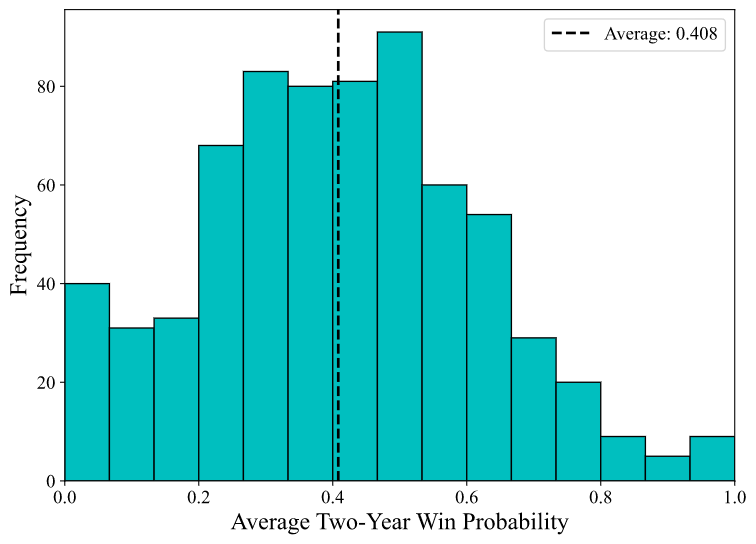
\includegraphics[width=1\linewidth]{hist1.png}}
\caption{Average two-year win probability distribution.}
\label{fig2}
\end{figure}

\begin{figure}[htbp]
\centerline{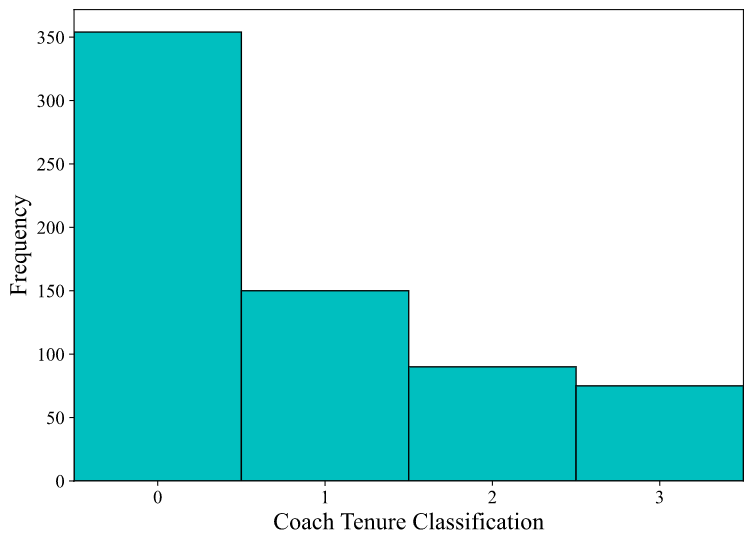
\includegraphics[width=1\linewidth]{hist2.png}}
\caption{Coach tenure classification distribution.}
\label{fig3}
\end{figure}

Fig. \ref{fig3} shows a histogram of coach tenure classification for all head coach hires in the history of the NFL. This figure shows that the data is imbalanced, with frequency of class decreasing with increasing coach tenure. It should be noted that this histogram does not include any currently active head coaches hired during or since 2014, as there has not been enough time for these coaches to be correctly and definitively labeled.

\section{Results}
For all models and all implementations, the data was split into training and validation sets via an 80/20 ratio. Each model was created using multiple levels of internal cross-validation in order to tune hyperparameters. This section reports performance metrics on the training set, the testing set, and the validation set. The testing set is the set of data set aside within internal cross-validation during hyperparameter tuning. The validation set is the 20\% of the entire set that was not used in any portion of training. Do not confuse the testing set and the validation set. Final claims of model performance are made on performance with the validation set.

\subsection{Predicting Average Two-Year Winning Probability}

\subsubsection{Linear Regression with Lasso Regularization}
This implementation used an outer ten-fold cross-validation over an inner five-fold cross-validation, each iterating over $1,000$ values of the regularization parameter alpha, to determine the hyperparameter value with the best model performance. Following this cross-validation, a single model was built on the entirety of the training set and used to test the validation set. Table \ref{tab2} shows the hyperparameter value with best average performance. 

\begin{table}[htbp]
\caption{Regularized Linear Regression Hyperparameter Values}
\begin{center}
\begin{tabular}{|c||c|}
\hline
\textbf{Hyperparameter} & \textbf{Value} \\
\hline
\hline
Alpha & 0.001 \\
\hline
\end{tabular}
\label{tab2}
\end{center}
\end{table}

\begin{table}[htbp]
\caption{Regularized Linear Regression RMSE Results}
\begin{center}
\begin{tabular}{|c||c|}
\hline
\textbf{Data Set} & \textbf{RMSE} \\
\hline
\hline
Train & 0.197 \\
\hline
Test & 0.202 \\
\hline
Validation & 0.202 \\
\hline
Validation, Expected Outcome$^{\mathrm{1}}$ & 0.208 \\
\hline
\multicolumn{2}{l}{$^{\mathrm{1}}$Not influenced by the model.}
\end{tabular}
\label{tab3}
\end{center}
\end{table}

\begin{figure}[htbp]
\centerline{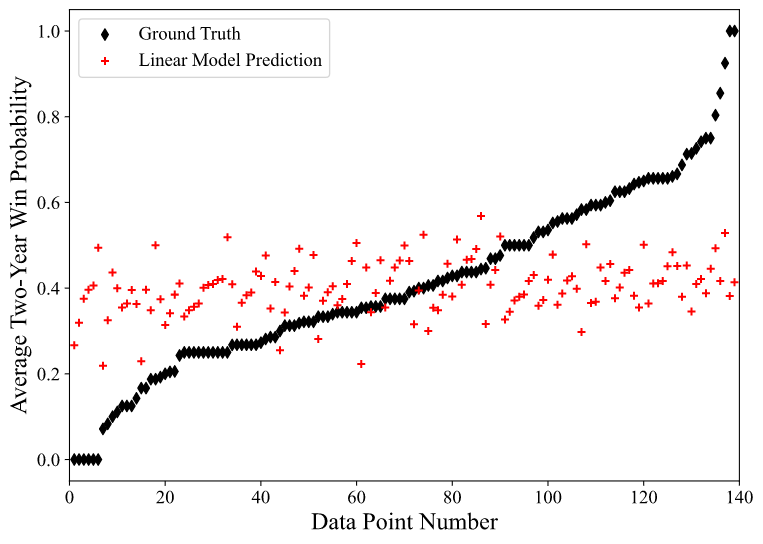
\includegraphics[width=1\linewidth]{test1.png}}
\caption{Validation set, regularized linear model prediction versus ground truth.}
\label{fig4}
\end{figure}

Table \ref{tab3} shows the results of this implementation. These results show that the regularized linear regression performed marginally better on the validation set than predicting the expected value for the validation set. Fig. \ref{fig4} shows the sorted validation set with corresponding marks for the ground truth values and the predicted values. Fig. \ref{fig4} shows that the regularized linear model tends to predict winning probabilities near the expected value. Additionally, the model's variance in predicted probability is far less than the variance in the validation set. 

\begin{figure}[htbp]
\centerline{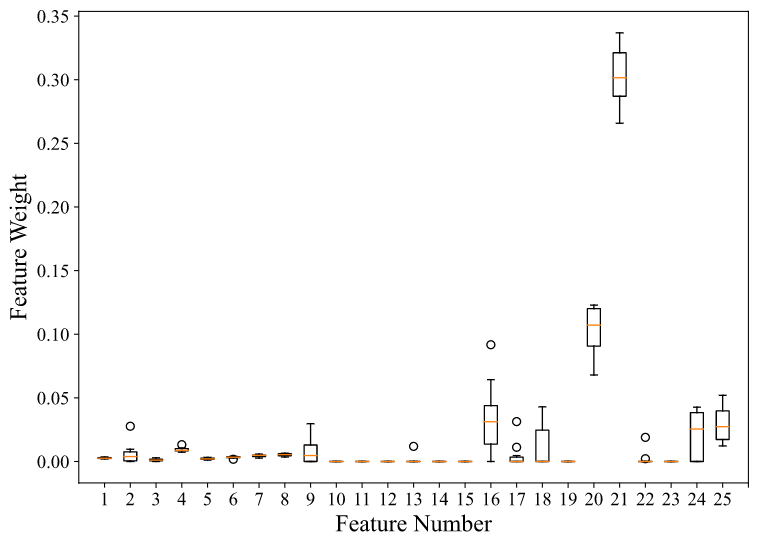
\includegraphics[width=1\linewidth]{weight1.png}}
\caption{Regularized linear model feature weight distributions.}
\label{fig5}
\end{figure}

Fig. \ref{fig5} shows the feature weight distributions resulting from the best models found within the outer ten-fold cross-validation. These weights show that on average, the regularization set seven feature weights to zero and twelve additional weights to less than $0.01$. This regularization left six features with appreciable weight, listed in decreasing importance: features 21, 20, 16, 25, 24, and 18. Only two of these features, 16 and 18, are features specific to the coaching candidate. The remaining four features are all measures of team success prior to the coaching hire. 

These findings suggest that the coach-specific features in the model are not linearly related to the win probability of the coach. This model further suggests that characteristics of the team prior to coach hiring are most important when attempting to predict future win probability in a linear model.

\subsubsection{XGBoost Regressor}
This implementation used an outer ten-fold cross-validation over an inner five-fold cross-validation, each iterating over $4,032$ hyperparameter sets to determine the configuration with the best performance. Following this cross-validation, a single model was built on the entirety of the training set and used to test the validation set. Table \ref{tab4} shows the hyperparameter set with best average performance. Table \ref{tab5} shows the results of this implementation.

\begin{table}[htbp]
\caption{XGBoost Regressor Hyperparameter Values}
\begin{center}
\begin{tabular}{|c||c|}
\hline
\textbf{Hyperparameter} & \textbf{Value} \\
\hline
\hline
Objective & reg:squarederror \\
\hline
Number of Estimators & 100 \\
\hline
Learning Rate & 0.05 \\
\hline
Max Estimator Depth & 10 \\
\hline
Gamma & 0.1 \\
\hline
Alpha & 0 \\
\hline
\end{tabular}
\label{tab4}
\end{center}
\end{table}

\begin{table}[htbp]
\caption{XGBoost Regressor RMSE Results}
\begin{center}
\begin{tabular}{|c||c|}
\hline
\textbf{Data Set} & \textbf{RMSE} \\
\hline
\hline
Train & 0.154 \\
\hline
Test & 0.204 \\
\hline
Validation & 0.215 \\
\hline
Validation, Expected Outcome$^{\mathrm{1}}$ & 0.208 \\
\hline
\multicolumn{2}{l}{$^{\mathrm{1}}$Not influenced by the model.}
\end{tabular}
\label{tab5}
\end{center}
\end{table}

These results show that the XGBoost regressor had a worse RMSE than that of predicting the expected value. This finding is surprising, as cross-validated gradient boosting models typically perform well. The low RMSE of the train set shows that this implementation may have overfit the data, leading to poor generalization on non-training data. The cause of this over-fitting is not known, as two levels of cross-validation encompassed hyperparameter searching.

Fig. \ref{fig6} shows the sorted validation set with corresponding marks for the ground truth values and the predicted values.  Fig. \ref{fig6} shows that the XGBoost regressor model tends to predict winning probabilities near the expected value. This model has more variance in its predicted values than the regularized linear model. 

\begin{figure}[htbp]
\centerline{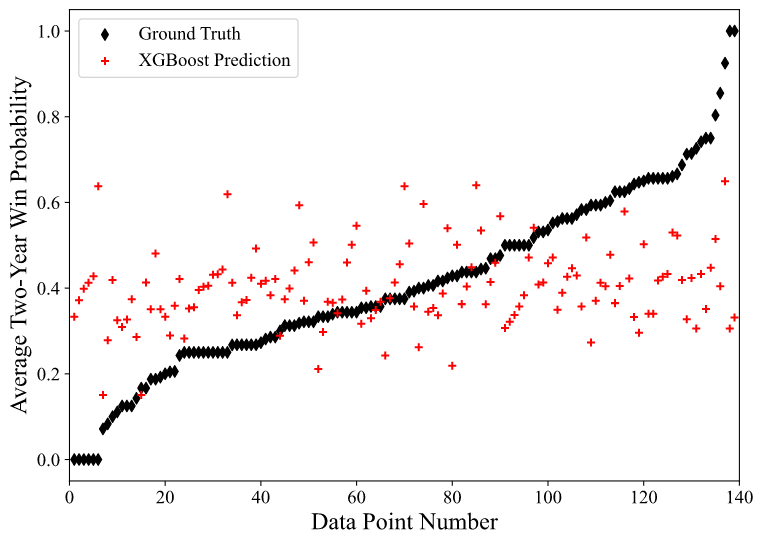
\includegraphics[width=1\linewidth]{test2.png}}
\caption{Validation set, XGBoost regresssor prediction versus ground truth.}
\label{fig6}
\end{figure}

Fig. \ref{fig7} shows the feature weight distributions resulting from the best models found within the outer ten-fold cross-validation. These weights show that on average, most features have similar importance. If all features had an equal weight, the weight would be $\frac{1}{25}=0.04$. Fig. \ref{fig7} shows that ten features have an importance greater than this value. These features in decreasing order of importance are: 19, 21, 20, 17, 8, 12, 22, 23, 14, and 4. Five of these features are team metrics, and five of these features are coach metrics. 

\begin{figure}[htbp]
\centerline{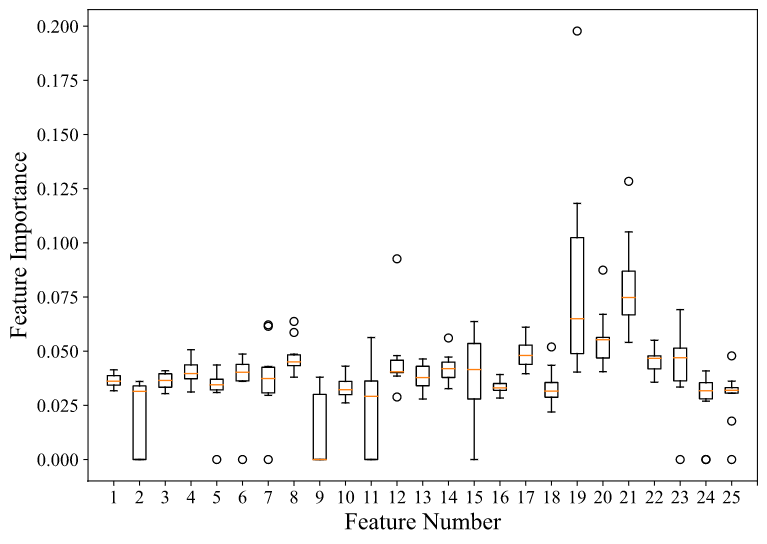
\includegraphics[width=1\linewidth]{weight2.png}}
\caption{XGBoost regressor feature weight distributions.}
\label{fig7}
\end{figure}

Unlike the linear model, these feature importance values cannot be interpreted as correlating directly with the model prediction. This restriction is a result of the weak learning unit: a tree. Trees make predictions based on sequential data partitions based on threshold values in individual features. Thus, the aggregation of multiple trees creates ranges of feature values, each with a different impact on the prediction. These findings suggest that a boosted tree-based learning model is not adequate to predict the average two year win probabilities of head coach hires. The final model's roughly equal feature weights and the equal proportion of coach and team metrics within the set of important features suggests that there is no underlying pattern or relationship that explains these win probabilities.

\subsubsection{Multi-layer Perceptron Regressor}
This implementation used an outer ten-fold cross-validation over an inner five-fold cross-validation, each iterating over $72$ hyperparameter sets to determine the configuration with the best performance. Following this cross-validation, a single model was built on the entirety of the training set and used to test the validation set. Table \ref{tab6} shows the hyperparameter set with best average performance. Table \ref{tab7} shows the results of this implementation.

\begin{table}[htbp]
\caption{MLP Regressor Hyperparameter Values}
\begin{center}
\begin{tabular}{|c||c|}
\hline
\textbf{Hyperparameter} & \textbf{Value} \\
\hline
\hline
Activation & relu \\
\hline
Solver & lbfgs \\
\hline
Alpha & 0 \\
\hline
Hidden Layer Sizes & (50, 25) \\
\hline
Max Iterations & 200 \\
\hline
Tolerance & $1e^{-5}$ \\
\hline
\end{tabular}
\label{tab6}
\end{center}
\end{table}

\begin{table}[htbp]
\caption{MLP Regressor RMSE Results}
\begin{center}
\begin{tabular}{|c||c|}
\hline
\textbf{Data Set} & \textbf{RMSE} \\
\hline
\hline
Train & 0.194 \\
\hline
Test & 0.212 \\
\hline
Validation & 0.199 \\
\hline
Validation, Expected Outcome$^{\mathrm{1}}$ & 0.208 \\
\hline
\multicolumn{2}{l}{$^{\mathrm{1}}$Not influenced by the model.}
\end{tabular}
\label{tab7}
\end{center}
\end{table}

These results show that the MLP regressor had the best performance of any implementation on the validation set. Nonetheless, the high validation RMSE value further supports the observation in previous models that these features are not sufficient to accurately predict the average winning probability. Fig. \ref{fig8} shows the sorted validation set with corresponding marks for the ground truth values and the predicted values.  Fig. \ref{fig8} shows that the MLP regressor tends to predict winning probabilities near the expected value. 

\begin{figure}[htbp]
\centerline{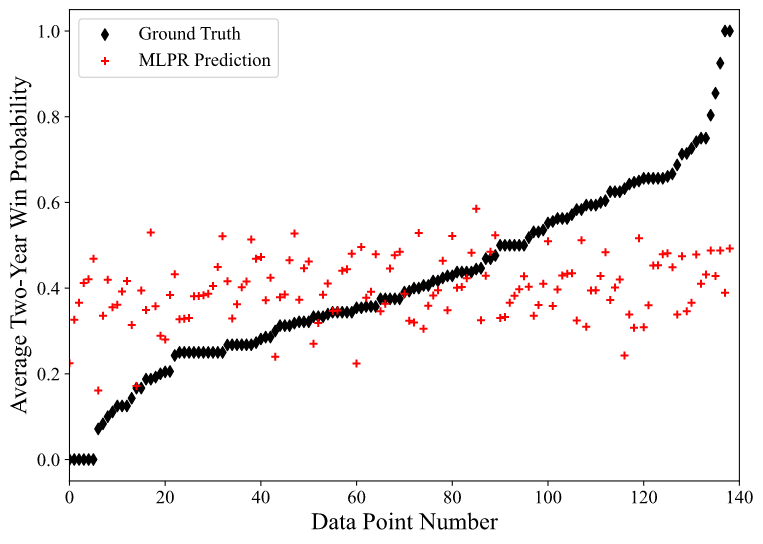
\includegraphics[width=1\linewidth]{test3.png}}
\caption{Validation set, MLP regresssor prediction versus ground truth.}
\label{fig8}
\end{figure}

Unlike the previous two implementations, neural networks do not have a simple or straightforward means to measure feature importance. This project uses Local Surrogate Interpretable Machine Learning (LIME) to analyze the final MLP model to estimate feature weights \cite{b9}. Fig. \ref{fig9} shows the feature weight distributions resulting from LIME. It should be noted that unlike the previous feature weight distributions, these weights are associated with permutations of individual data points within the validation set, rather than the outer cross-validation.

\begin{figure}[htbp]
\centerline{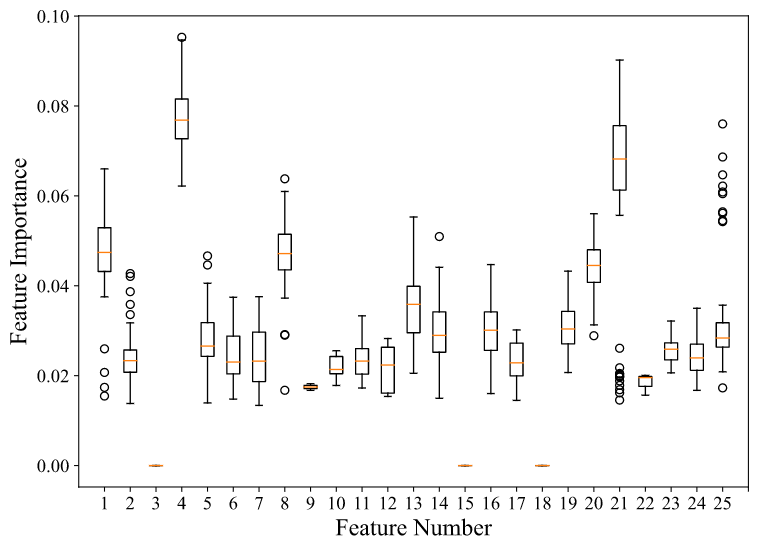
\includegraphics[width=1\linewidth]{weight3.png}}
\caption{MLP regressor feature weight distributions from LIME.}
\label{fig9}
\end{figure}

These weights show significantly more feature importance variance than either previous implementation. Fig. \ref{fig9} shows that five features have an importance greater than the high importance threshold of $0.04$. In decreasing order of importance, these features are: 4, 21, 8, 1, and 20. Two of these features are team metrics, and three of these features are coach metrics. Additionally, this feature analysis also shows that two features associated with team turnovers, features 15 and 18, have no importance.

\subsubsection{Comparison}
Table \ref{cum1} compares the results of these three implementations. This table shows that the MLP regressor had the best performance on the validation set. All models showed poor RMSE performance when compared to predicting the expected value. These findings suggest that these features, largely driven by characteristics of the head coach, are not sufficient to predict a team's winning probability. In other words, it appears that a head coach hire will not drive a change in win probability based on these features.

\begin{table}[htbp]
\caption{Winning Probability Prediction Result Comparison}
\begin{center}
\begin{tabular}{|c||c|c|c|}
\hline
\textbf{Data} & \multicolumn{3}{|c|}{\textbf{RMSE}}\\
\cline{2-4} 
\textbf{Set} & \textbf{Reg. Lin.} &  \textbf{XGBR} &  \textbf{MLPR} \\
\hline
\hline
Train & 0.197 & 0.154 & 0.194\\
\hline
Test & 0.202 & 0.204 & 0.212 \\
\hline
Validation & 0.202 & 0.215 & 0.199 \\
\hline
Validation, Expected Outcome$^{\mathrm{1}}$ & \multicolumn{3}{|c|}{0.208} \\
\hline
\multicolumn{2}{l}{$^{\mathrm{1}}$Not influenced by any model.}
\end{tabular}
\label{cum1}
\end{center}
\end{table}

\subsection{Predicting Coach Tenure Classification}

\subsubsection{Logistic Regression with Lasso Regularization}
This implementation used an outer ten-fold cross-validation over an inner five-fold cross-validation, each iterating over $9$ values of the regularization parameter $C$, to determine the hyperparameter value with the best model performance. Following this cross-validation, a single model was built on the entirety of the training set and used to test the validation set. Table \ref{tab8} shows the hyperparameter value with best average performance. 

\begin{table}[htbp]
\caption{Regularized Logistic Regression Hyperparameter Values}
\begin{center}
\begin{tabular}{|c||c|}
\hline
\textbf{Hyperparameter} & \textbf{Value} \\
\hline
\hline
C & 0.01 \\
\hline
\end{tabular}
\label{tab8}
\end{center}
\end{table}

\begin{table}[htbp]
\caption{Regularized Logistic Regression OVR AUROC Results}
\begin{center}
\begin{tabular}{|c||c|}
\hline
\textbf{Data Set} & \textbf{OVR AUROC} \\
\hline
\hline
Train & 0.629 \\
\hline
Test & 0.577 \\
\hline
Validation & 0.605 \\
\hline
Validation, Expected Outcome$^{\mathrm{1}}$ & 0.500 \\
\hline
\multicolumn{2}{l}{$^{\mathrm{1}}$Not influenced by the model.}
\end{tabular}
\label{tab9}
\end{center}
\end{table}

\begin{figure}[htbp]
\centerline{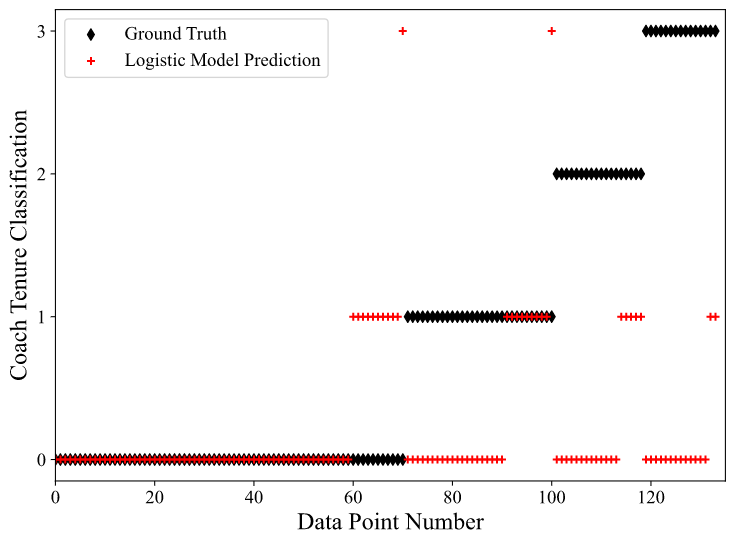
\includegraphics[width=1\linewidth]{test4.png}}
\caption{Validation set, regularized logistic regression prediction versus ground truth.}
\label{fig10}
\end{figure}

Table \ref{tab9} shows the results of this implementation. These results show that the regularized logistic regression performed  appreciably better on the validation set than predicting the expected value for the validation set. Fig. \ref{fig10} shows the sorted validation set with corresponding marks for the ground truth values and the predicted values. Fig. \ref{fig10} shows that the logistic model does not appear to distinguish class two from the other classes, as no points in the validation set were predicted in class two. Additionally, these results show that the model tends to predict class zero for a significant portion of the validation set. 

\begin{figure}[htbp]
\centerline{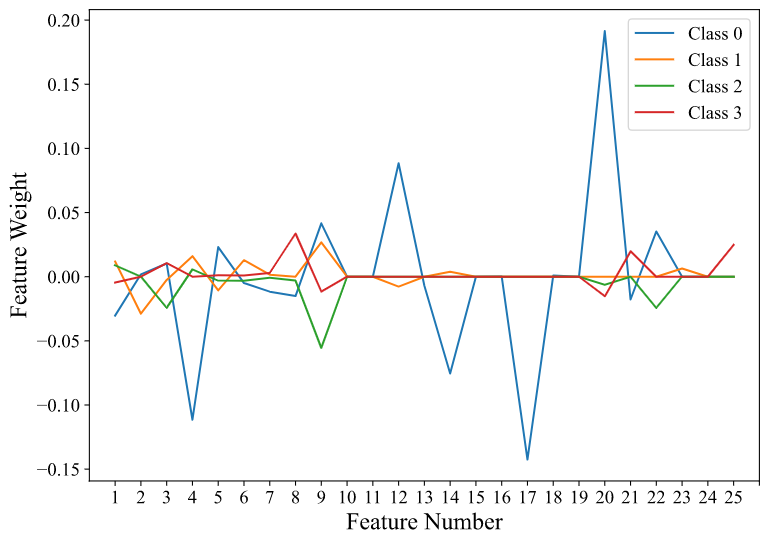
\includegraphics[width=1\linewidth]{weight4.png}}
\caption{Regularized logistic regression feature weight distributions.}
\label{fig11}
\end{figure}

A multi-class logistic regression with $k$ classes is the culmination of $k$ OVR classifiers. As a result, a multi-class logistic regression has $k$ sets of coefficients, one for each OVR classifier. Fig. \ref{fig11} shows the average feature weights for each OVR classifier over the outer cross-validation. For any class and any feature, a positive weight signifies that increasing the feature value increases the probability of the point being the class. Conversely, a negative weight signifies that increasing the feature value decreases the probability of the point being the class. 

Fig. \ref{fig11} shows that the coach metric with the greatest impact on predicting class zero is feature 17, the team's average normalized point differential rank during years as a head coach. Thus, this model suggests that head coaches with better average normalized point differential ranks in their coaching history are more likely to have greater tenure as a head coach. 

A notable related finding is that features 25 and 21, the hiring team's number of playoff appearances and average normalized point differential rank in previous two seasons, have the second and third largest impact on predicting class three, respectively. This finding suggests that successful teams are more likely to have head coaches with longer tenures, independent of characteristics of the head coach hired. This claim may infer that successful teams are better at evaluating head coaching candidates. 

\subsubsection{XGBoost Classifier}
This implementation used an outer ten-fold cross-validation over an inner five-fold cross-validation, each iterating over $1,200$ hyperparameter sets to determine the configuration with the best performance. Following this cross-validation, a single model was built on the entirety of the training set and used to test the validation set. Table \ref{tab11} shows the hyperparameter set with best average performance. Table \ref{tab12} shows the results of this implementation.

\begin{table}[htbp]
\caption{XGBoost Classifier Hyperparameter Values}
\begin{center}
\begin{tabular}{|c||c|}
\hline
\textbf{Hyperparameter} & \textbf{Value} \\
\hline
\hline
Objective & multi:softprob \\
\hline
Number of Estimators & 25 \\
\hline
Learning Rate & 0.2 \\
\hline
Max Estimator Depth & 2 \\
\hline
Gamma & 0 \\
\hline
Lambda & 0 \\
\hline
\end{tabular}
\label{tab11}
\end{center}
\end{table}

\begin{table}[htbp]
\caption{XGBoost Classifier OVR AUROC Results}
\begin{center}
\begin{tabular}{|c||c|}
\hline
\textbf{Data Set} & \textbf{OVR AUROC} \\
\hline
\hline
Train & 0.905 \\
\hline
Test & 0.634 \\
\hline
Validation & 0.706 \\
\hline
Validation, Expected Outcome$^{\mathrm{1}}$ & 0.500 \\
\hline
\multicolumn{2}{l}{$^{\mathrm{1}}$Not influenced by the model.}
\end{tabular}
\label{tab12}
\end{center}
\end{table}

These results show that the XGBoost classifier has a significantly better performance on the validation set than the regularized logistic regression. The OVR AUROC value of $0.706$ shows that the model has predictive utility. Fig. \ref{fig12} shows the sorted validation set with corresponding marks for the ground truth values and the predicted values. These results show that like the logistic regression, this model was not able to distinguish classes two and three. Unlike the logistic regression, this model predicted class two rather than class three. 

\begin{figure}[htbp]
\centerline{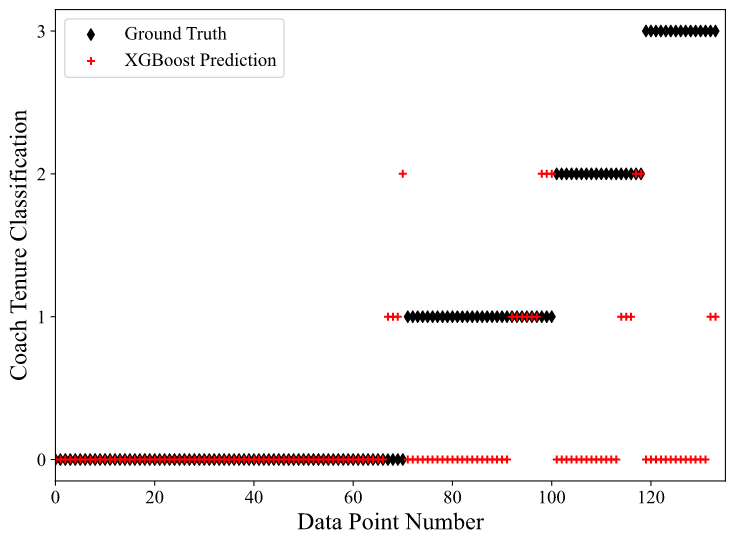
\includegraphics[width=1\linewidth]{test5.png}}
\caption{Validation set, XGBoost classifier prediction versus ground truth.}
\label{fig12}
\end{figure}

Fig. \ref{fig13} shows the feature weight distributions resulting from the best models found within the outer ten-fold cross-validation. Unlike the logistic regression, these feature importance do not infer a monotonic relationship between feature value and predicted value. Rather, these importance distributions result from feature prevalence in the model's weak estimators. A feature with higher importance is present in more estimators than a feature with low importance. 

\begin{figure}[htbp]
\centerline{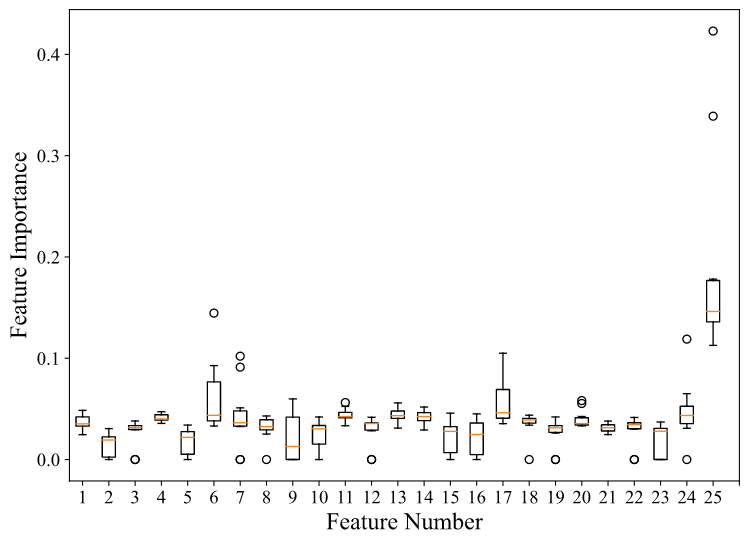
\includegraphics[width=1\linewidth]{weight5.png}}
\caption{XGBoost classifier feature weight distributions.}
\label{fig13}
\end{figure}

These weights are tightly clustered, with only one feature with outlying importance. This feature is 25, the hiring team's number of playoff wins in the previous two years. This feature's distinct importance suggests that a successful team impacts coach hiring tenure. Thus, this model also suggests that successful franchises may be better at evaluating coaching candidates. 

\subsubsection{Multi-layer Perceptron Classifier}
This implementation used an outer ten-fold cross-validation over an inner five-fold cross-validation, each iterating over $32$ hyperparameter sets to determine the configuration with the best performance. Following this cross-validation, a single model was built on the entirety of the training set and used to test the validation set. Table \ref{tab13} shows the hyperparameter set with best average performance. Table \ref{tab14} shows the results of this implementation.

\begin{table}[htbp]
\caption{MLP Classifier Hyperparameter Values}
\begin{center}
\begin{tabular}{|c||c|}
\hline
\textbf{Hyperparameter} & \textbf{Value} \\
\hline
\hline
Activation & relu \\
\hline
Hidden Layer Sizes & (100) \\
\hline
Max Iterations & 200 \\
\hline
Tolerance & $1e^{-4}$ \\
\hline
Alpha & 0.001 \\
\hline
\end{tabular}
\label{tab13}
\end{center}
\end{table}

\begin{table}[htbp]
\caption{MLP Classifier OVR AUROC Results}
\begin{center}
\begin{tabular}{|c||c|}
\hline
\textbf{Data Set} & \textbf{OVR AUROC} \\
\hline
\hline
Train & 0.752 \\
\hline
Test & 0.579 \\
\hline
Validation & 0.704 \\
\hline
Validation, Expected Outcome$^{\mathrm{1}}$ & 0.500 \\
\hline
\multicolumn{2}{l}{$^{\mathrm{1}}$Not influenced by the model.}
\end{tabular}
\label{tab14}
\end{center}
\end{table}

These results show that the MLP classifier performed slightly worse than the XGBoost model on the validation set. Nonetheless, the performance is a significant improvement over the expected outcome. Fig. \ref{fig14} shows the sorted validation set with corresponding marks for the ground truth values and the predicted values. These results show that the MLP classifier is more willing to predict data points in classes one, two, and three, as compared to the previous two implementations. Like the previous models, this model does not distinguish classes two and three well. 

\begin{figure}[htbp]
\centerline{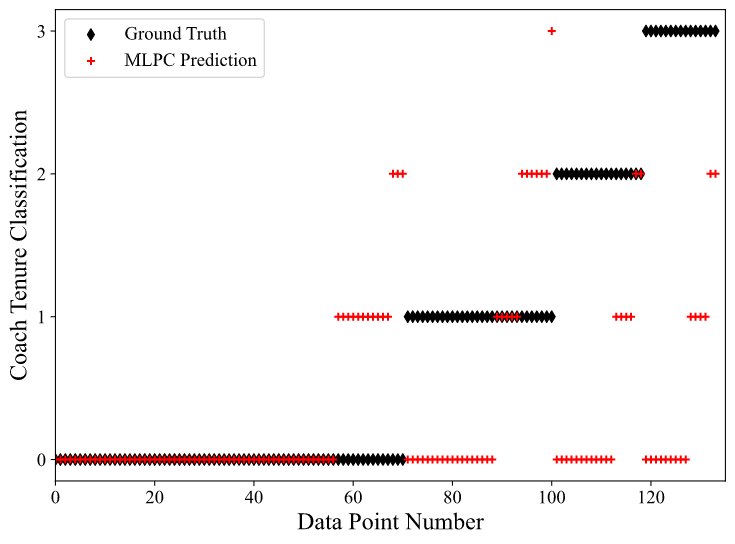
\includegraphics[width=1\linewidth]{test6.png}}
\caption{Validation set, MLP classifier prediction versus ground truth.}
\label{fig14}
\end{figure}

Similar to the MLP regressor, the MLP classifier does not have straightforward feature weights. Once again, LIME is used to estimate feature weight distributions over the validation set. Fig. \ref{fig15} shows this estimate. These feature weights differ greatly than the weights in the previous models, as ten of the twelve most important features are coach metrics. These results suggest that the neural network approaches coach hiring classification similar to how franchises approach hiring decisions: by focusing on experience and performance in prior positions. Feature 19, the hiring team's average winning percentage in the previous two years, had no importance in this model. This result is suprising, as it shows the MLP classifier does not believe this feature impacts coach hire tenure.

\begin{figure}[htbp]
\centerline{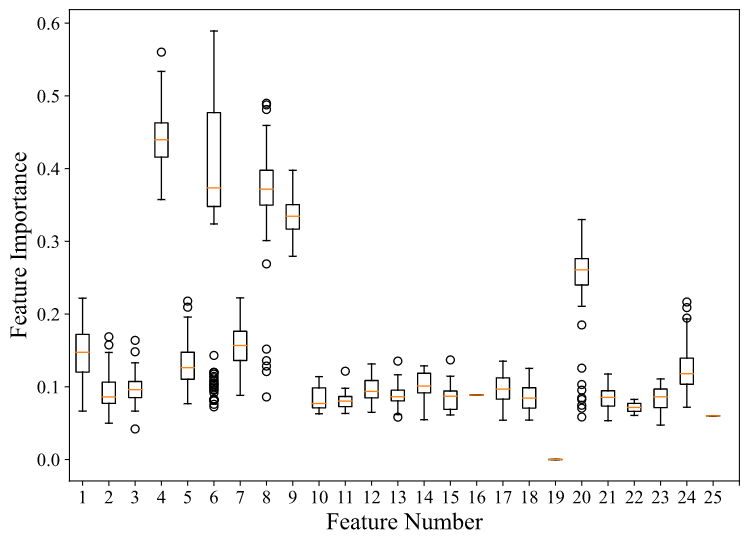
\includegraphics[width=1\linewidth]{weight6.png}}
\caption{MLP classifier feature weight distributions from LIME.}
\label{fig15}
\end{figure}

\begin{table}[htbp]
\caption{MLP Classifier Class Two and Three Predictions}
\begin{center}
\begin{tabular}{|c||c|c|c|c|}
\hline
\textbf{Coach} & \textbf{Hire} & \textbf{True} & \textbf{Pred.} & \textbf{2nd Pred.} \\
\textbf{Name} & \textbf{Year} & \textbf{Class} & \textbf{Class} & \textbf{Class} \\
\hline
\hline
Red Strader & 1948 & 0 & 2 & 1 \\
\hline
Howard Schnellenberger & 1973 & 0 & 2 & 3 \\
\hline
Tom Fears & 1967 & 1 & 2 & 0 \\
\hline
Dirk Koetter & 2016 & 1 & 2 & 1 \\
\hline
Mike Singletary & 2009 & 1 & 2 & 1 \\
\hline
Bill Parcells & 1993 & 1 & 2 & 1 \\
\hline
Gus Bradley & 2013 & 1 & 2 & 1 \\
\hline
Bill Parcells & 1997 & 1 & 2 & 3 \\
\hline
Chuck Knox & 1992 & 1 & 3 & 0 \\
\hline
Bill Parcells & 2003 & 1 & 3 & 1 \\
\hline
Jack Pardee & 1990 & 2 & 2 & 0 \\
\hline
Bum Phillips & 1981 & 2 & 2 & 1 \\
\hline
Mike Shanahan & 2016 & 3 & 2 & 3 \\
\hline
\end{tabular}
\label{tab15}
\end{center}
\end{table}

Table \ref{tab15} lists all coaches predicted with tenure two or three by the MLP classifier. Although there are some notable misses, like Howard Schnellenberger, there are also impressive predictions, such as Mike Shanahan's hire with the Broncos, which lead to two Super Bowl victories. These predictions should lend some sense of realism to the model's predictions. 

\subsubsection{Comparison}
Table \ref{cum2} compares the results of these three implementations. This table shows that the XGBoost classifier had the best performance on the validation set. All models showed better performance when compared to predicting the expected value. These findings suggest that these features, largely driven by characteristics of the head coach, do have some value in predicting the tenure of head coaches. 

\begin{table}[htbp]
\caption{Coach tenure Classification Prediction Result Comparison}
\begin{center}
\begin{tabular}{|c||c|c|c|}
\hline
\textbf{Data} & \multicolumn{3}{|c|}{\textbf{OVR AUROC}}\\
\cline{2-4} 
\textbf{Set} & \textbf{Reg. Log.} &  \textbf{XGBC} &  \textbf{MLPC} \\
\hline
\hline
Train & 0.629 & 0.905 & 0.752\\
\hline
Test & 0.577 & 0.634 & 0.579 \\
\hline
Validation & 0.605 & 0.706 & 0.704 \\
\hline
Validation, Expected Outcome$^{\mathrm{1}}$ & \multicolumn{3}{|c|}{0.500} \\
\hline
\multicolumn{2}{l}{$^{\mathrm{1}}$Not influenced by any model.}
\end{tabular}
\label{cum2}
\end{center}
\end{table}

\section{Limitations and Future Directions}
The development of these models required many assumptions and limitations in design. One of the most impactful decisions made in this project was to use linearly distributed values to normalize feature ranks across eras. This decision simplified data creation, but may have removed important variance from the data set. For example, the current approach does not preserve the magnitude of the difference in performance metrics. The difference between a $n$ place team with $2k$ value and a $n+1$ place team with a $k$ value is the same as the difference between a $n$ place team with $k+1$ value and a $n+1$ place team with a $k$ value. This lost difference in performance could provide additional utility in model prediction. Future work could use a $Z$ score distance from league average for these average normalized features to increase the variance in the data while still respecting differences in statistics among different eras.

Future work could also benefit from more advanced neural networks. In both predictions, the neural networks performed impressively well on the validation set considering their simplicity. More advanced neural networks could perform better unsupervised feature extraction to provide better predictive utility. Future work could also repeat these analyses without the inclusion of interim coaches. 

\section{Conclusions}
This project attempted to predict the two-year winning probability and the coach tenure classification of all head coaches in NFL history. The three implementations of the winning probability prediction model showed poor performance when compared to predicting the expected value. The best RMSE value was $0.199$, equivalent to predicting the number of won games in a 16 game season to within $\pm3.18$ wins. Thus, these implementations have no practical predictive utility. These findings suggest that the features in this project, largely driven by characteristics of the head coach, are not sufficient to predict a team's winning probability. In other words, it appears that a head coach hire will not drive a change in win probability based on these features.

Implementation of three models to predict coach tenure classification showed significantly better performance than predicting the most prevalent class. Both the XGBoost and the MLP classifiers had similar OVR AUROC values of $0.706$ and $0.704$, respectively. Although these models had significantly different feature weights, their performance shows that the features in this project, largely driven by characteristics of the head coach, do have some ability to predict the tenure of head coach hires. All models had some trouble distinguishing between classes two and three, suggesting that there may not be an appreciable difference in the characteristics of coaches that belong to each class. Additionally, the regularized logistic regression and the XGBoost classifier showed that characteristics of successful hiring teams were important in determining coaches with longer tenures, suggesting that successful franchises may be better at evaluating head coach candidates. Regardless, future iterations of these models could provide significant value to NFL franchises by increasing the likelihood of successful head coach hires.

\begin{thebibliography}{00}
\bibitem{b1} T. Barrabi, ``What is the NFL worth? Revenue, team values and other financial facts,'' Fox Business. https://www.foxbusiness.com/sports/nfl-worthrevenue-team-values (accessed Oct. 26, 2020)
\bibitem{b2} C. Gaines, ``NFL head coaches have good job security when compared to other major sports leagues,'' Business Insider. https://www.businessinsider.com/coaches-managers-tenure-nfl-mlb-nba-nhl-premier-league-2016-12 (accessed Oct. 26, 2020)
\bibitem{b3} ``How does a change in CEO impact stock price?,'' Investopedia. https://www.investopedia.com/ask/answers/010815/how-does-change-ceo-impact-stock-price.asp (accessed Nov. 18, 2020)
\bibitem{b4} ``Using machine learning to peek inside the minds of NFL coaches,'' DataRobot. https://www.datarobot.com/blog/using-machine-learning-to-peek-inside-the-minds-of-nfl-coaches/ (accessed Oct. 26, 2020)
\bibitem{b5} M. Roach, ``Does prior NFL head coaching experience improve team performance?,'' in Journal of Sport Management, vol. 30, no. 3, pp. 298-311.
\bibitem{b6} D. Mielke, ``Coaching experience, playing experience, and coaching tenure: a commentary,'' in International Journal of Sports Science \& Coaching, vol. 2, no. 2, pp. 117-118.
\bibitem{b7} Pedregosa et al., ``Scikit-learn: machine learning in Python,'' in Journal of Machine Learning Research, vol. 12, pp.2825-2830.
\bibitem{b8} T. Chen, and C. Guestrin, ``XGBoost: a scalable tree boosting system,'' in KDD '16: Proceedings of the 22nd ACM SIGKDD International Conference on Knowledge Discovery and Data Mining, pp.785-794.
\bibitem{b9} M. Ribeiro, S. Singh, and C. Guestrin, ````Why should I trust you?'': Explaining the predictions of any classifier,'' in KDD '16: Proceedings of the 22nd ACM SIGKDD International Conference on Knowledge Discovery and Data Mining, pp.1135-1144.
\end{thebibliography}

\end{document}
